\subsection{Fake Source Injection for DIA}
\subsubsection{Selection of a data subset}

We selected a subset of 24 visits chosen from observations processed by the DRP pipelines that included image
subtraction, in order to learn about DIA performance, as well as that of the detection and measurement
algorithms.

We chose visits with a zenith distance of less than 45 degrees, as well as some technical parameters, derived from the nominal DRP DIA performance (ratio of PSF between template and science, as well as Kernel basis condition number). 

We create a catalog of fakes for these visits by injecting synthetic sources near true sources which are
possibly extended, and with a flux within 1.5 magnitudes of the selected source host
(\figRef{scatter_radec_diaSrcs_match_arsec_mag})

\begin{figure}
    \centering
    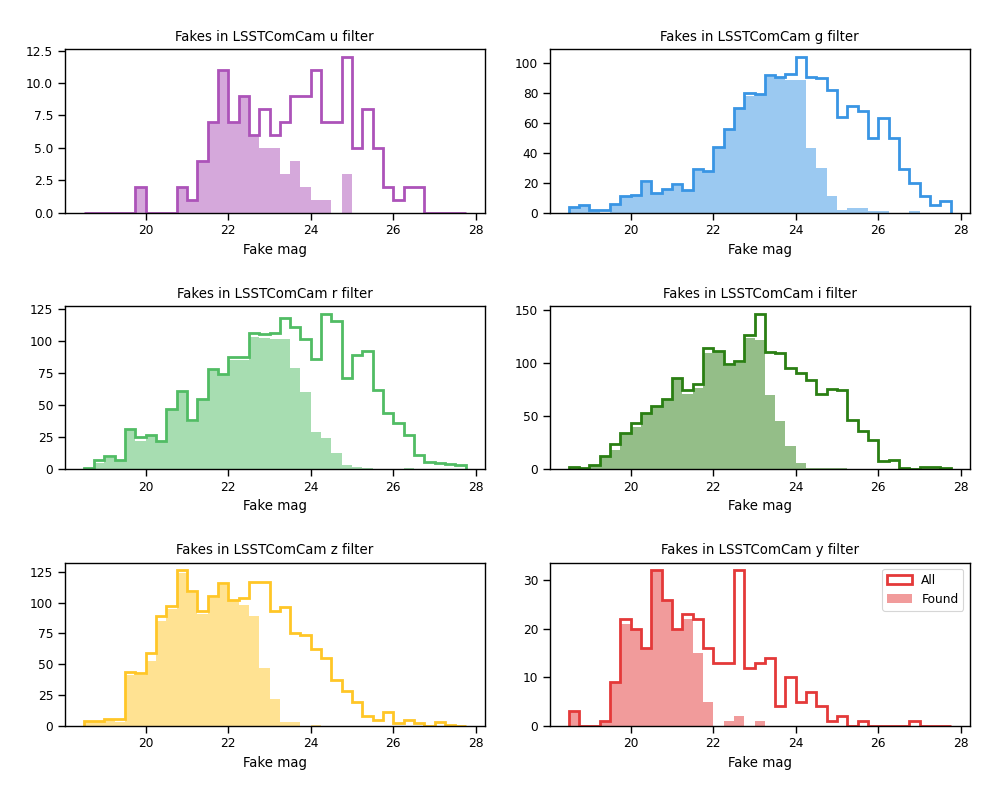
\includegraphics[width=0.5\linewidth]{dia/figures/simple_hist_completeness_mag_per_filter.png}
    \caption{The distribution of magnitudes per bandpass for all the injected fakes (solid lines), and in shaded region the distribution of magnitudes of the fakes detected by the AP pipeline.}
    \label{fig:found_fakes_per_Filter}
\end{figure}


We run Alert Production pipeline with a set of additional tasks that handle fake injection on the
\texttt{initial\_pvi} images, and then the book-keeping tasks of fake catalog matching to diaSources as well
as forced photometry for SNR estimation. We then cross-matched the position of our candidate detections, or
\textit{diaSources} with the positions of the synthetic sources, using a tolerance of $0.5''$ (roughly
$2.5$px).

Those fakes that found a match are called ``found fake'' and objects that had no match we refer as ``lost'' or
``missed'' fakes.  The rate of found to existing fakes is our recovery rate, Recall or Efficiency of detection.

\begin{figure}
    \centering
    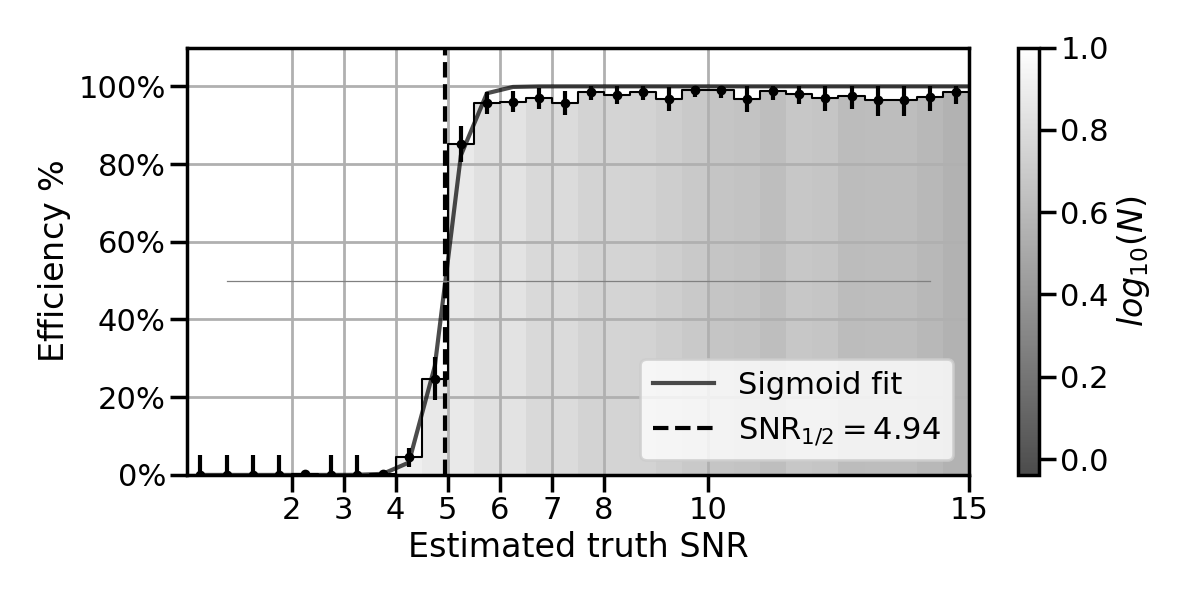
\includegraphics[width=0.95\linewidth]{dia/figures/Efficiency_vs_forced_base_PsfFlux_instFlux_SNR.png}
    \caption{The detection efficiency as function of the PSF estimated S/N ratio of the fake sources. The SNR 1/2 parameter is also included in dashed lines, and represents the 50\% efficiency S/N threshold value (lower is better).}
    \label{fig:eff_vs_snr_fakes}
\end{figure}

\begin{figure}
    \centering
    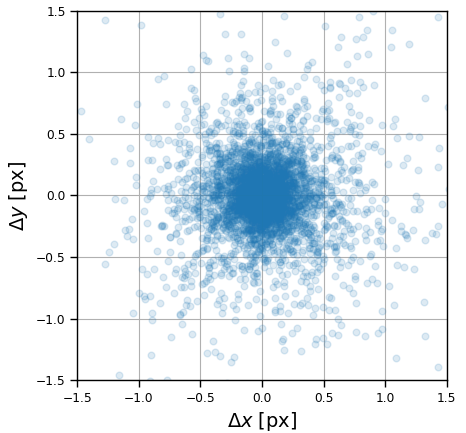
\includegraphics[height=0.3\textheight]{dia/figures/scatter_xy_diaSrcs_match_px.png}
    \hfil
    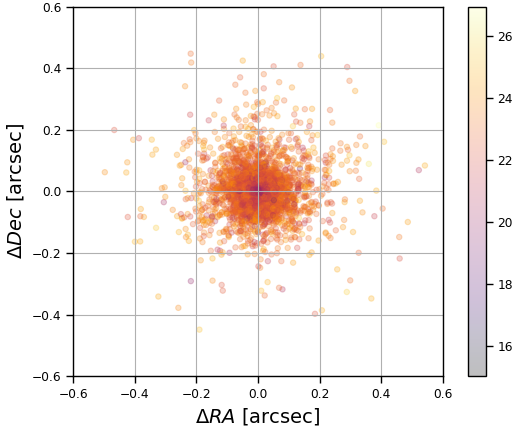
\includegraphics[height=0.3\textheight]{dia/figures/scatter_radec_diaSrcs_match_arsec_mag.png}
    \caption{The scatter of the coordinate centroid recovery of the fakes. In the left we have the scatter around the true centroid in pixel coordinates, and in the right the scatter around the true center of fakes in sky coordinates (and in units of arc-seconds), wit the grid matching the pixel grid by means of the platescale. Also, we include the brightness in colormap.}
    \label{fig:scatter_radec_diaSrcs_match_arsec_mag}
\end{figure}

\iffalse                                % doesn't add much to the PSF mags, and has more scatter
\begin{figure}
    \centering
    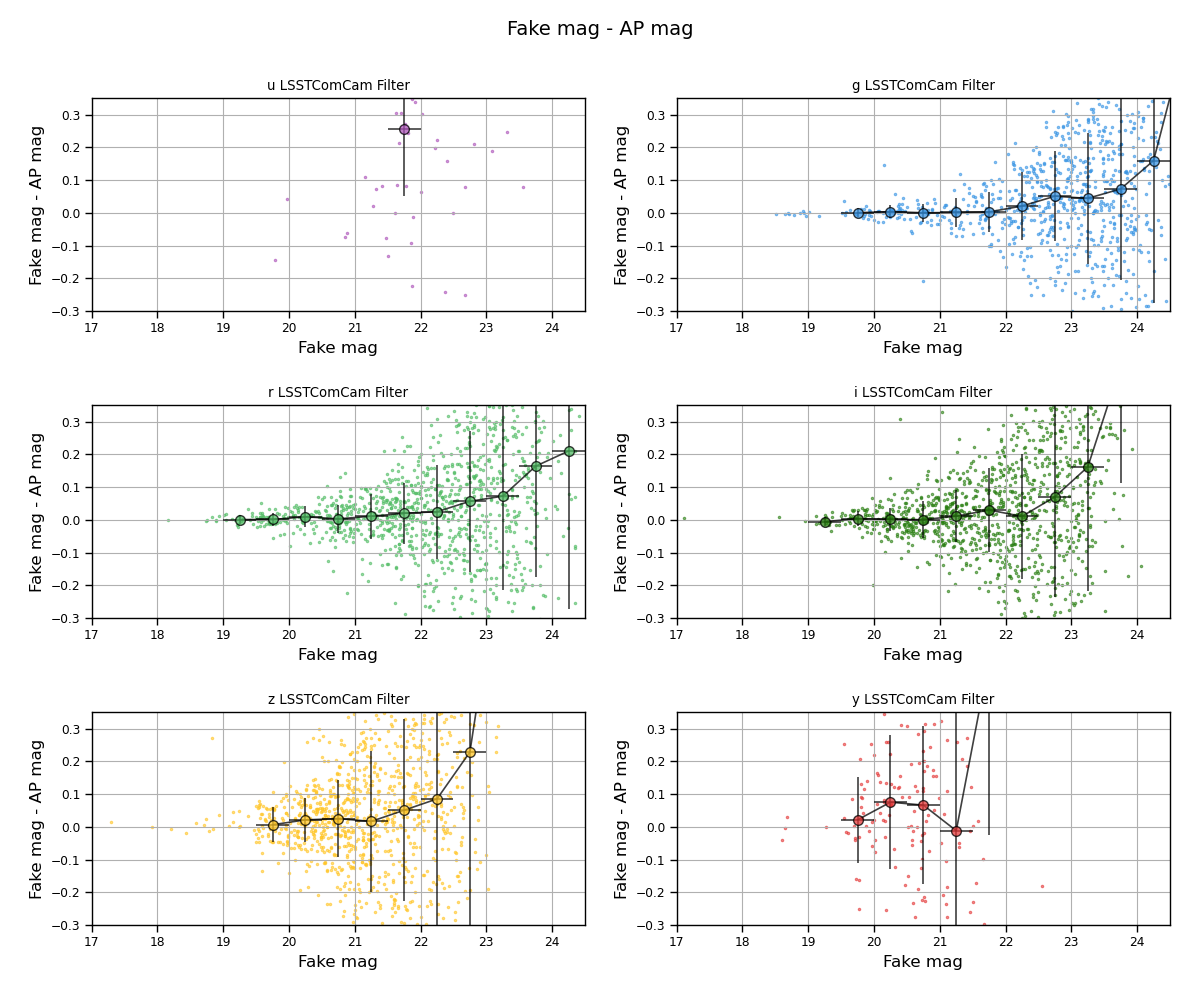
\includegraphics[width=0.95\linewidth]{dia/figures/scatter_mag_ap_mag_perfilter.png}
    \caption{The recovered Aperture magnitude residual per filter for all the found fake sample, as a function of their true magnitude. }
    \label{fig:photometric_recovery_vs_fakemag}
\end{figure}
\fi

\begin{figure}
    \centering
    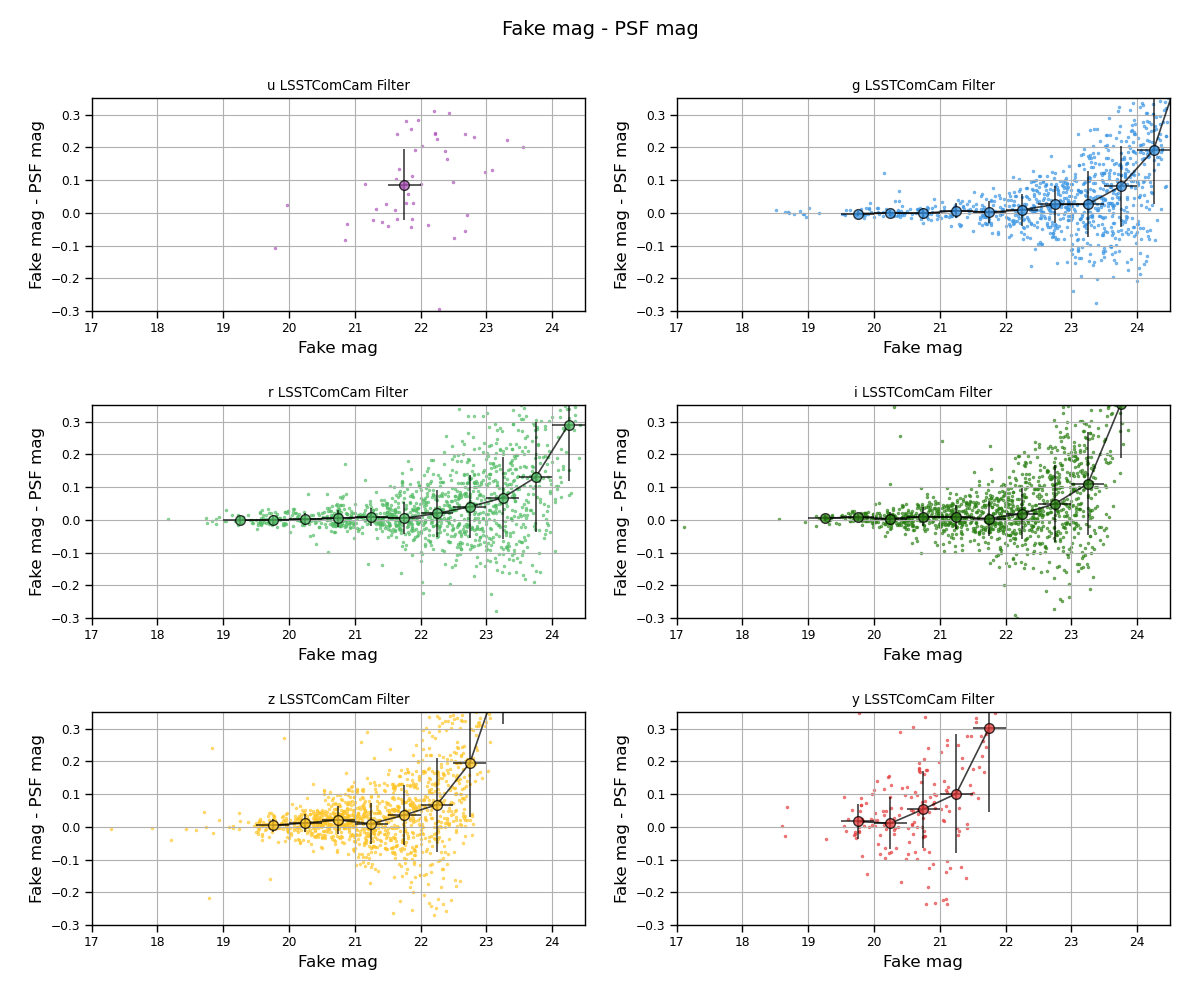
\includegraphics[width=0.45\textwidth]{dia/figures/scatter_mag_psf_mag_perfilter.png}
    \hfil
    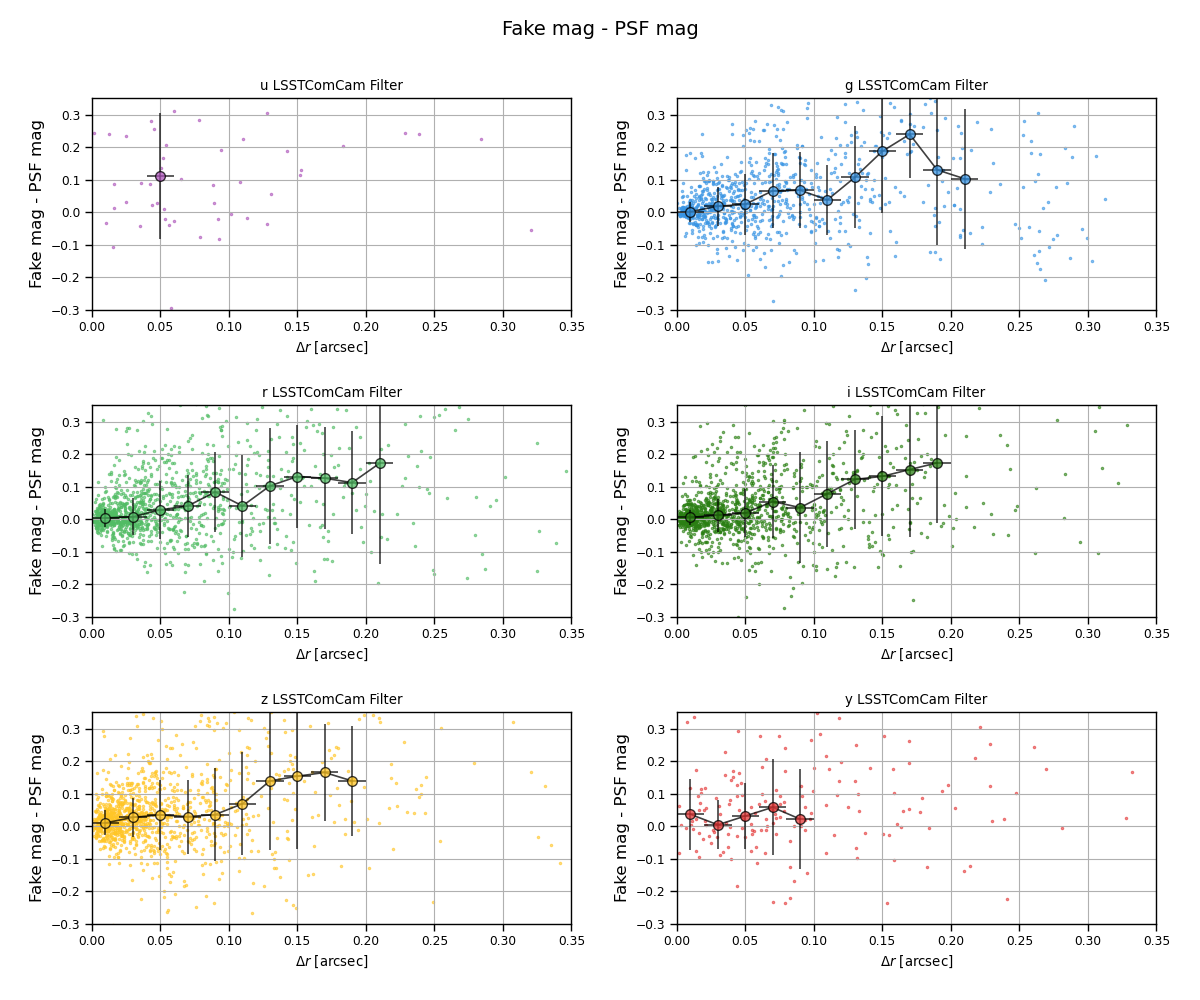
\includegraphics[width=0.45\textwidth]{dia/figures/scatter_dist_psf_mag_perfilter.png}
    \caption{The residual of PSF magnitude measurement for found fakes, as function of their true magnitude
    (left) or matching distance in arcsec (right).}
    \label{fig:dia_photometric_recovery}
\end{figure}

\iffalse                                % Needs to be analysed as a function of flux
\begin{figure}
    \centering
    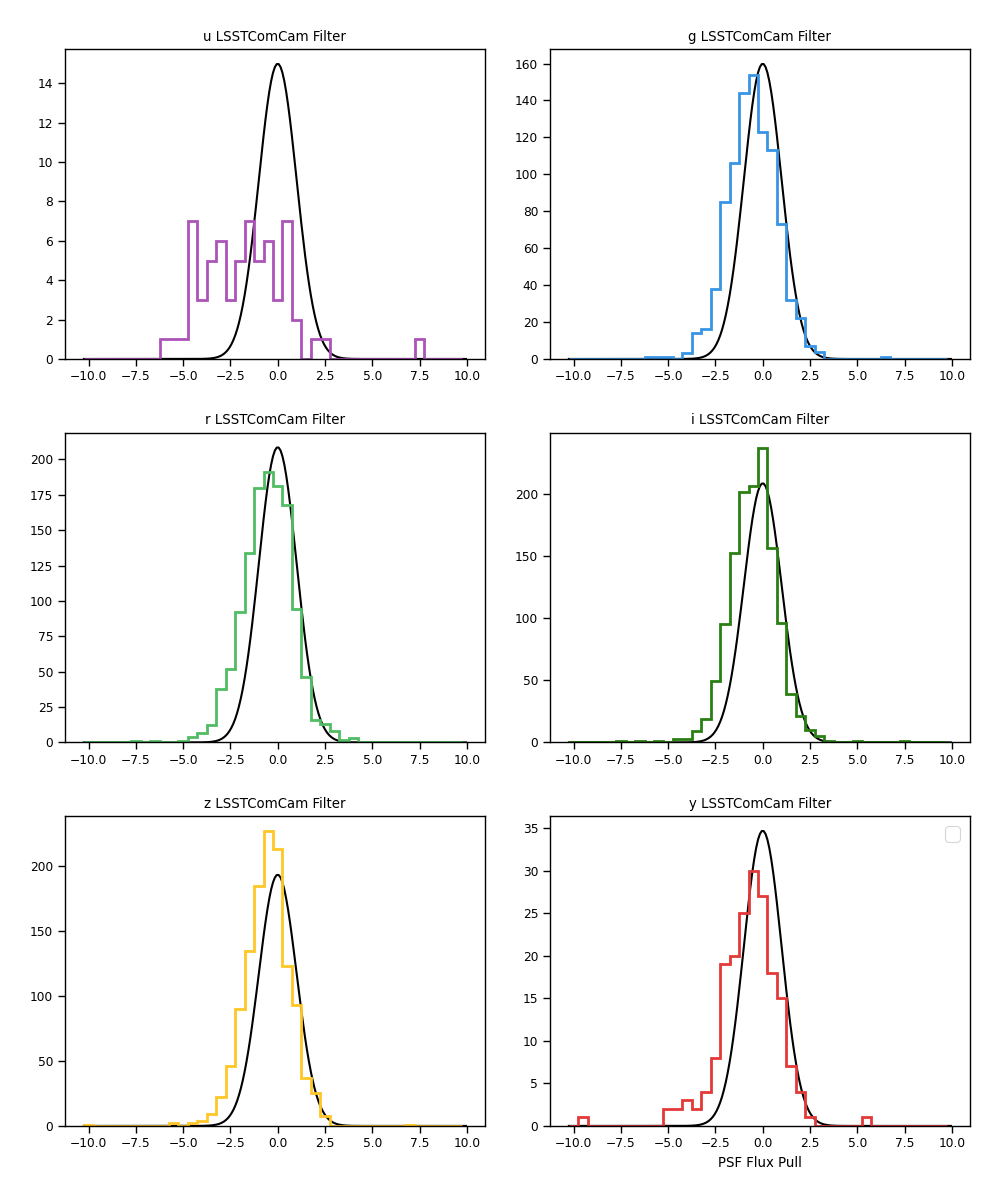
\includegraphics[width=0.95\linewidth]{dia/figures/flux_pulls.png}
    \caption{The flux pull (``$\chi$'') distribution for all the found fakes, in each filter bandpass. A zero mean, unit dispersion Gaussian distribution function is also included for reference.}
    \label{fig:fake_sources_pulls}
\end{figure}
\fi

\iffalse                                % what does this tell us?
\begin{figure}
    \centering
    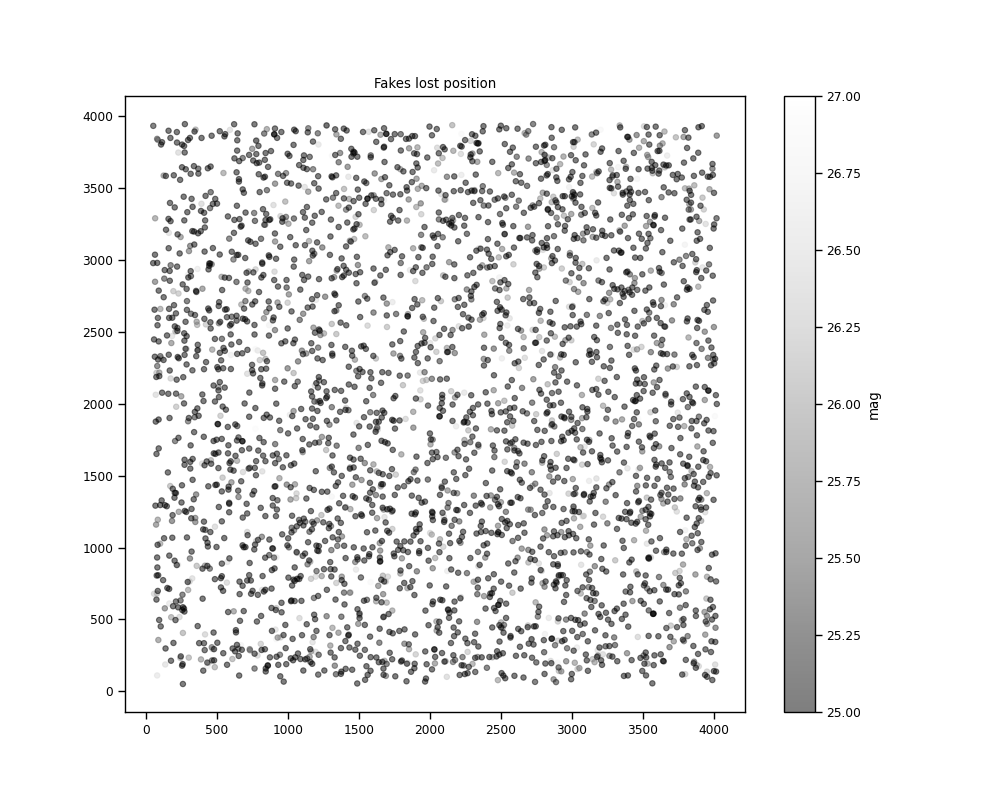
\includegraphics[width=0.95\linewidth]{dia/figures/lost_sources_detector_map.png}
    \caption{The scatter map of the lost sources in the detector coordinates. In gray scale in the colorbar we show the object magnitudes.}
    \label{fig:lost_sources_xy}
\end{figure}
\fi

The detection efficiency is plotted in \figRef{eff_vs_snr_fakes}; 
the astrometric errors in the recovered synthetic sources is shown in
\figRef{scatter_radec_diaSrcs_match_arsec_mag}, while the photometric errors appear
in \figRef{dia_photometric_recovery}
